\begin{wrapfigure}[2]{r}[-1cm]{3cm}
 \vspace{-6cm}
  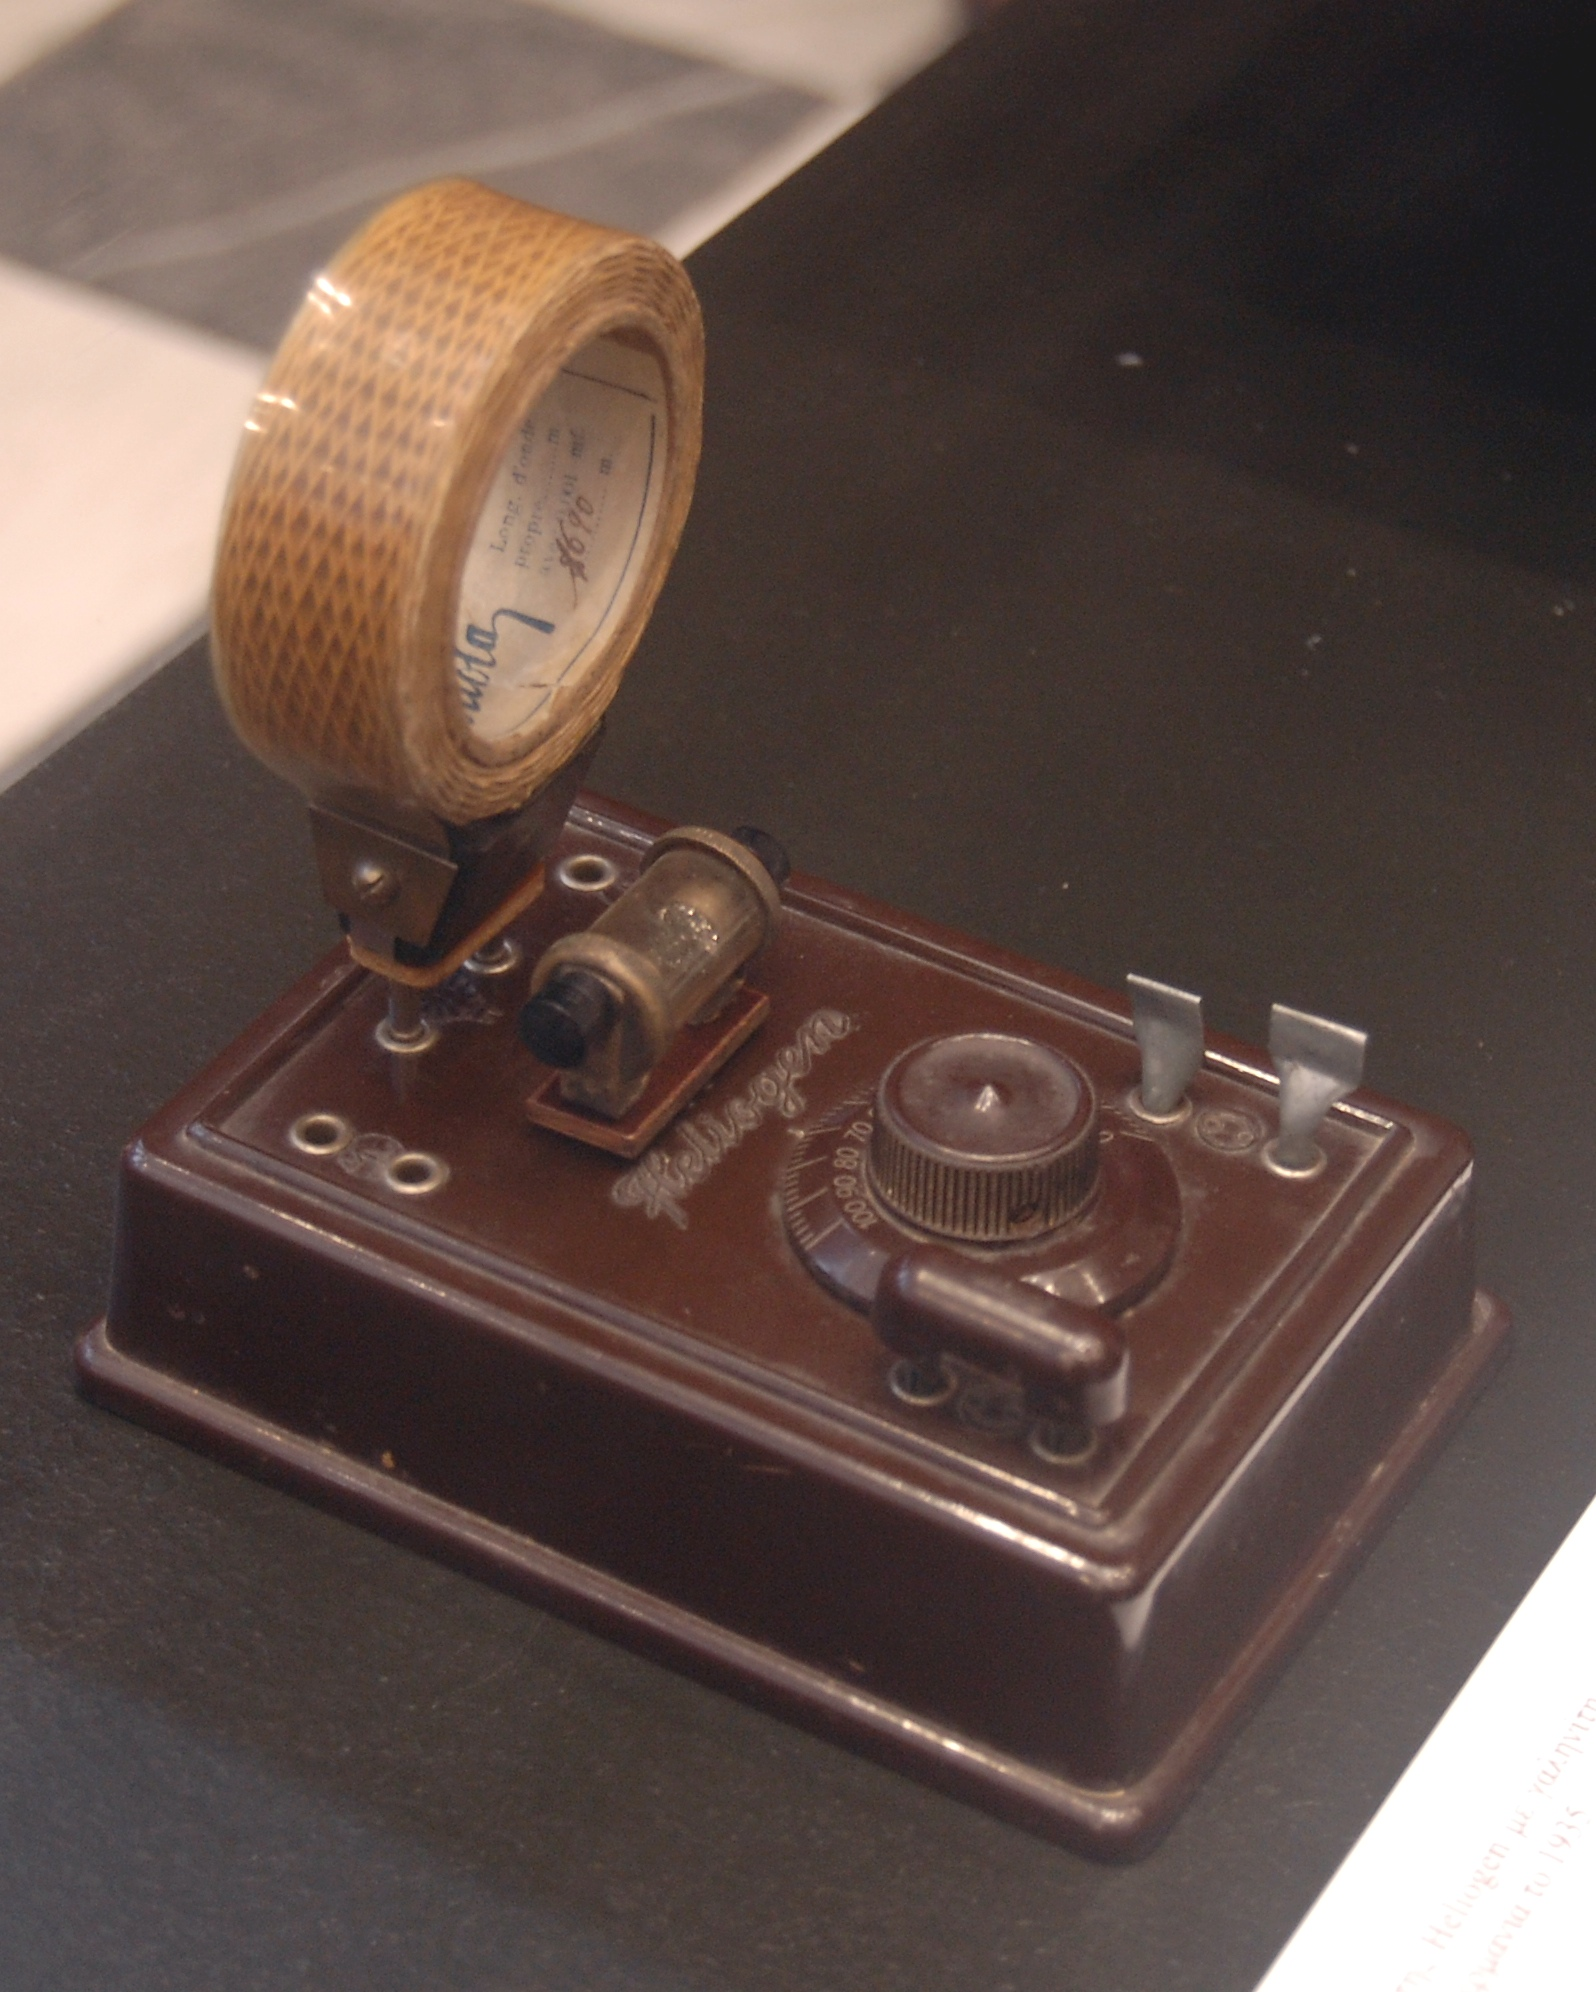
\includegraphics[scale=0.1]{Kurzwellendetektor/Bilder/Heliogen_medium_wave_galena_radio.JPG}
  %\caption{Historischer Detektorempfänger der Firma Heliogen (Deutschland 1935)}
 \vspace{-6cm}
\end{wrapfigure}

\section*{Praktische Anwendung}

Radio- und Funk-Signale empfangen ohne die Verwendugn einer Batterie oder einer anderen Energiequelle? Eine einfache Schaltung ermöglicht das. Die folgende Schaltung eines Detektorempfängers ist die einfachste aller Radioschaltungen. In der Frühzeit der Radiotechnik war das Konzept eines Detektorempfänger durchaus verbreitet. Heute ist es leider nich mehr ohne weiters möglich Radio-Sendungen mit dem der Kurzwellendetektor zu empfangen, da der großteil der Kurz- und Mittelwellensender ihren Betrieb eingestellt haben. Nichts desto tortz ist er ein guter Einstieg und ein technisches Abenteuer.


\begin{itemize}
\itemsep1pt\parskip0pt\parsep0pt
\item Baue folgende Schaltung auf (Abbildung \ref{kd}). 
\end{itemize}

\begin{figure}[H]
\centering
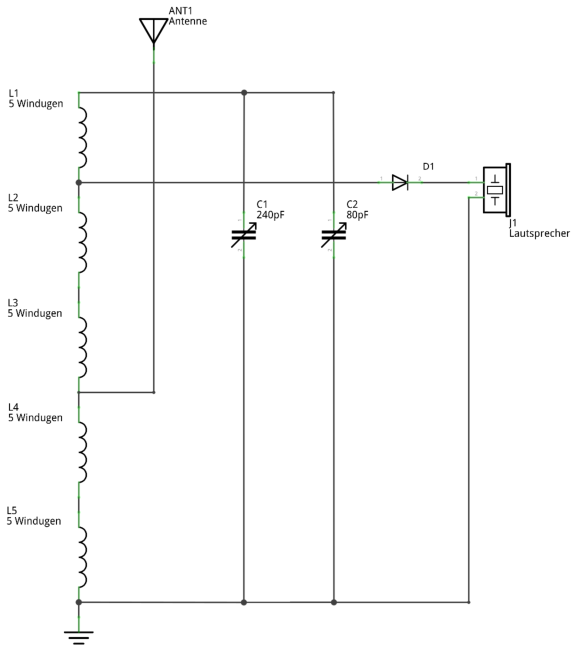
\includegraphics[scale=1.1]{Kurzwellendetektor/Schaltungen/Kurzwellendetektor_Schaltplan.pdf}
\caption{Der Kurzwellendetektor}
\label{kd}
\end{figure}